\begin{frame}{Algoritmos genecticos continuación}{Cap 4b p 12}
\begin{right}

Algoritmos geneticos requieren codificarse como cadenas (GPs usa programas)

La mezcla ayuda si las subcadenas son componentes significativos

\end{right}

\begin{center}
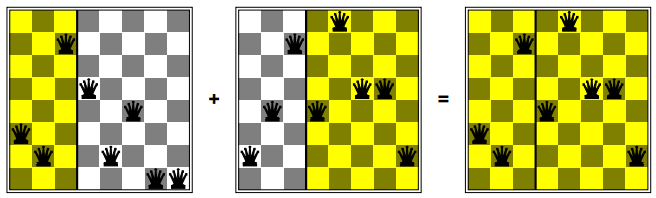
\includegraphics[scale = 0.4]{images/12p_4b.PNG}
\end{center}
\begin{right}

Algotirmos geneticos $ \neq $ evolucion: e.g., genes reales codifican maquinaria de replicación.

\end{right}
\end{frame}
